\section{System Design}
\graphicspath{ {./images/} }

\subsection{Objectives}
\par The system design objectives are:
\begin{itemize}
	\item Establish the final expected result as idea/sketch 
	\item Sketch the functionality scheme for each module needed in detail.
	\item Setup a server with the necessary dependencies.
	\item Setup a database used for storing user records
	\item Site mockup for: home page, plugin page, calendar page, login page, register page, account page
	\item Implement basic interactions between user and platform: registration, login, CRUD (create-read-update-delete) for records, implement calendar feature, import Google Calendar, add plugins
	\item Implement Companion feature.
	\item Create the possibility to add user-made plugins 
	\item Live testing and deployment.
	
\end{itemize}


\subsection{Requirements specification}
\par Requirements to this platform are:  
\begin{enumerate}
	\item Intuitive and easy to use design  
	
	\item Assistant which will companion the user all the time  
	
	\item FAQ page  
	
	\item User Friendly 
	
	\item Adaptive web design 
	
	\item Deep personalization 
	
	\item Seamlessly API integration. 
	
	\item Community custom made plugins. 
\end{enumerate}


\subsection{Full system design description. }
	\par Our solution consists of a variety of modules and components. As we adapted client-server architecture, we can divide the application in two parts, first client, which is visible by user, and strictly speaking is a gateway between user interaction with the server-side. Next one is server and it can be seen as the head of our app where most functionality is implemented. From user point of view, he/she enters the site (client), which sends requests to the server to fetch/insert some data from/into the database, do calculations etc. For instance, in Modular Organizer client is represented by front-end written in React JS (mostly on JSX) user can see it, interact and request something from the server. On the other hand, server consists of more than only back end. In summary, our back-end uses Python flask framework, Gunicorn application server,  Nginx and MySQL database.  
	
\subsection {System components description and motivation why selected system design fits the best solution for team selected problem. }
\par To realize our goals, we decided to create next components: 
	\begin{enumerate}
		\item Calendar API
		\item Plugin API  
		\item Weather API  
		\item Todo API 
		\item Configuration Component 
		\item Authentication/Authorization Component 
		\item User, Calendar, Plugin, Weather and Todo Entities.
		\item Companion component  
	\end{enumerate}
\par Firstly, we created three different API’s to get the highest flexibility and scalability from our application. Thanks to this design, we can easily distribute this project to team members and even better, any errors related to Calendar API side won’t get messed up with Weather API or Todo API. It results in more structured code, esthetically more beautiful endpoints and of course, it is easier to create updates, because if Todo API needs update, Weather API won’t need it.  
\par Configuration Component is a must for development control. Every application needs to set up environment variables and e.t.c., and for development and production they will differ. This is why there is a need in this specific component. 
\par Authentication/Authorization Component is created to handle authorization and authentication process which will be used on other components/API’s later.  
\par Entities are database components. By following database normalization principles, we created different entities which correspond to the API working with them. 



\subsection{System components interactions. Description of how system components interact with each other, which technologies and protocols are used and which data payload and data format is used for system intercommunication. }
\par Modular Organizer can be divided into client and server parts. Client consists of html/css, javascript (React JS) and server is represented by python, gunicorn, nginx and mysql. Backend is further divided into plugin, calendar, weather and todo API’s. All of this is working under REST architectural style, where data transmission is realized via JSON and HTTP protocols. As it is known, HTTP has a pretty wide range of methods, however our project mostly depends on GET, POST, PUT and DELETE methods. The biggest difference between these methods is their purpose and existence of payload in POST. So, strictly speaking our user interacts via client (front end) with server API’s, which uses Nginx and Gunicorn to work with HTTP and WSGI, where last of these is needed for python. For example, user wants to see his/her calendar records for this month on the website. Client makes GET request to the server endpoint under calendar API. As most calendars use ISO8601 standard for datetime representation (like YYYY-MM-DDTHH:MM:SSZ) and Odata V4 protocol to work with data our project has it implemented in our endpoints too. Then server gets this request, it seeks for the time boundaries of calendar records from query string. After, our server connects to the database, finds all suitable fields, packs it into JSON and creates a response with a status code 200 (OK), required headers and JSON in it. As our front end and back end is placed on two different subdomains, we have to additionally allow CORS. It is pretty important to mention that our project has fully working Authentication system which uses JWT (JSON Web Token) to create access and refresh httponly cookies. Also, it is well-known that cookies are vulnerable to CSRF attacks. So, we decided to implement CSRF Double Submit Cookie Pattern and we will also implement 2FA (Two-Factor Authentication) later on. Now let's speak more in-depth about techniques and technologies we used in our project. 
\par HTTP - Stands for "Hypertext Transfer Protocol." HTTP is the protocol used to transfer data over the web. It is part of the Internet protocol suite and defines commands and services used for transmitting webpage data.
\par HTTP - Stands for "Hypertext Transfer Protocol." HTTP is the protocol used to transfer data over the web. It is part of the Internet protocol suite and defines commands and services used for transmitting webpage data.
\par Some common HTTP status codes include: 
\begin{enumerate}
	\item 200 - successful request (the webpage exists) 
	\item 301 - moved permanently (often forwarded to a new URL) 
	\item 401 - unauthorized request (authorization required) 
	\item 403 - forbidden (access is not allowed to the page or directory) 
	\item 500 - internal server error (often caused by an incorrect server configuration) 
	\item 418 – I am a teapot. (client error response code indicates that the server refuses to brew coffee because it is, permanently, a teapot) 
\end{enumerate}
\par HTTP also defines commands such as GET and POST, which are used to handle form submissions on websites. The CONNECT command is used to facilitate a secure connection that is encrypted using SSL. Encrypted HTTP connections take place over HTTPS, an extension of HTTP designed for secure data transmissions. 
\par NOTE: URLs that begin with "http://" are accessed over the standard hypertext transfer protocol and use port 80 by default. URLs that start with "https://" are accessed over a secure HTTPS connection and often use port 443. 
\par JSON - an open standard file format, and data interchange format, that uses human-readable text to store and transmit data objects consisting of attribute–value pairs and array data types. It is a very common data format, with a diverse range of applications, such as serving as a replacement for XML in AJAX systems. 
REST - Representational state transfer is a software architectural style that defines a set of constraints to be used for creating Web services. Web services that conform to the REST architectural style, called RESTful Web services, provide interoperability between computer systems on the internet. 

Odata (Open Data Protocol) - is an OASIS standard that defines the best practice for building and consuming RESTful APIs. OData helps you focus on your business logic while building RESTful APIs without having to worry about the approaches to define request and response headers, status codes, HTTP methods, URL conventions, media types, payload formats and query options etc. OData also guides you about tracking changes, defining functions/actions for reusable procedures and sending asynchronous/batch requests etc. Additionally, OData provides facility for extension to fulfil any custom needs of your RESTful APIs. 

OData RESTful APIs are easy to consume. The OData metadata, a machine-readable description of the data model of the APIs, enables the creation of powerful generic client proxies and tools. Some of them can help you interact with OData even without knowing anything about the protocol. The following 6 steps demonstrate 6 interesting scenarios of OData consumption across different programming platforms. But if you are a non-developer and would like to simply play with OData, XOData is the best start for you. 

ISO8601 - is an international standard covering the exchange of date- and time-related data. It was issued by the International Organization for Standardization (ISO) and was first published in 1988. The purpose of this standard is to provide an unambiguous and well-defined method of representing dates and times, so as to avoid misinterpretation of numeric representations of dates and times, particularly when data is transferred between countries with different conventions for writing numeric dates and times. 

WSGI - stands for “Web Server Gateway Interface”. It is used to forward requests from a web server (such as Apache or NGINX) to a backend Python web application or framework. From there, responses are then passed back to the webserver to reply to the requestor. 

CORS - Cross-origin resource sharing is a mechanism that allows restricted resources on a web page to be requested from another domain outside the domain from which the first resource was served. A web page may freely embed cross-origin images, stylesheets, scripts, iframes, and videos. 

\subsection{UML Diagrams}
\subsubsection{Use case}
\par
\begin{figure}[h]
	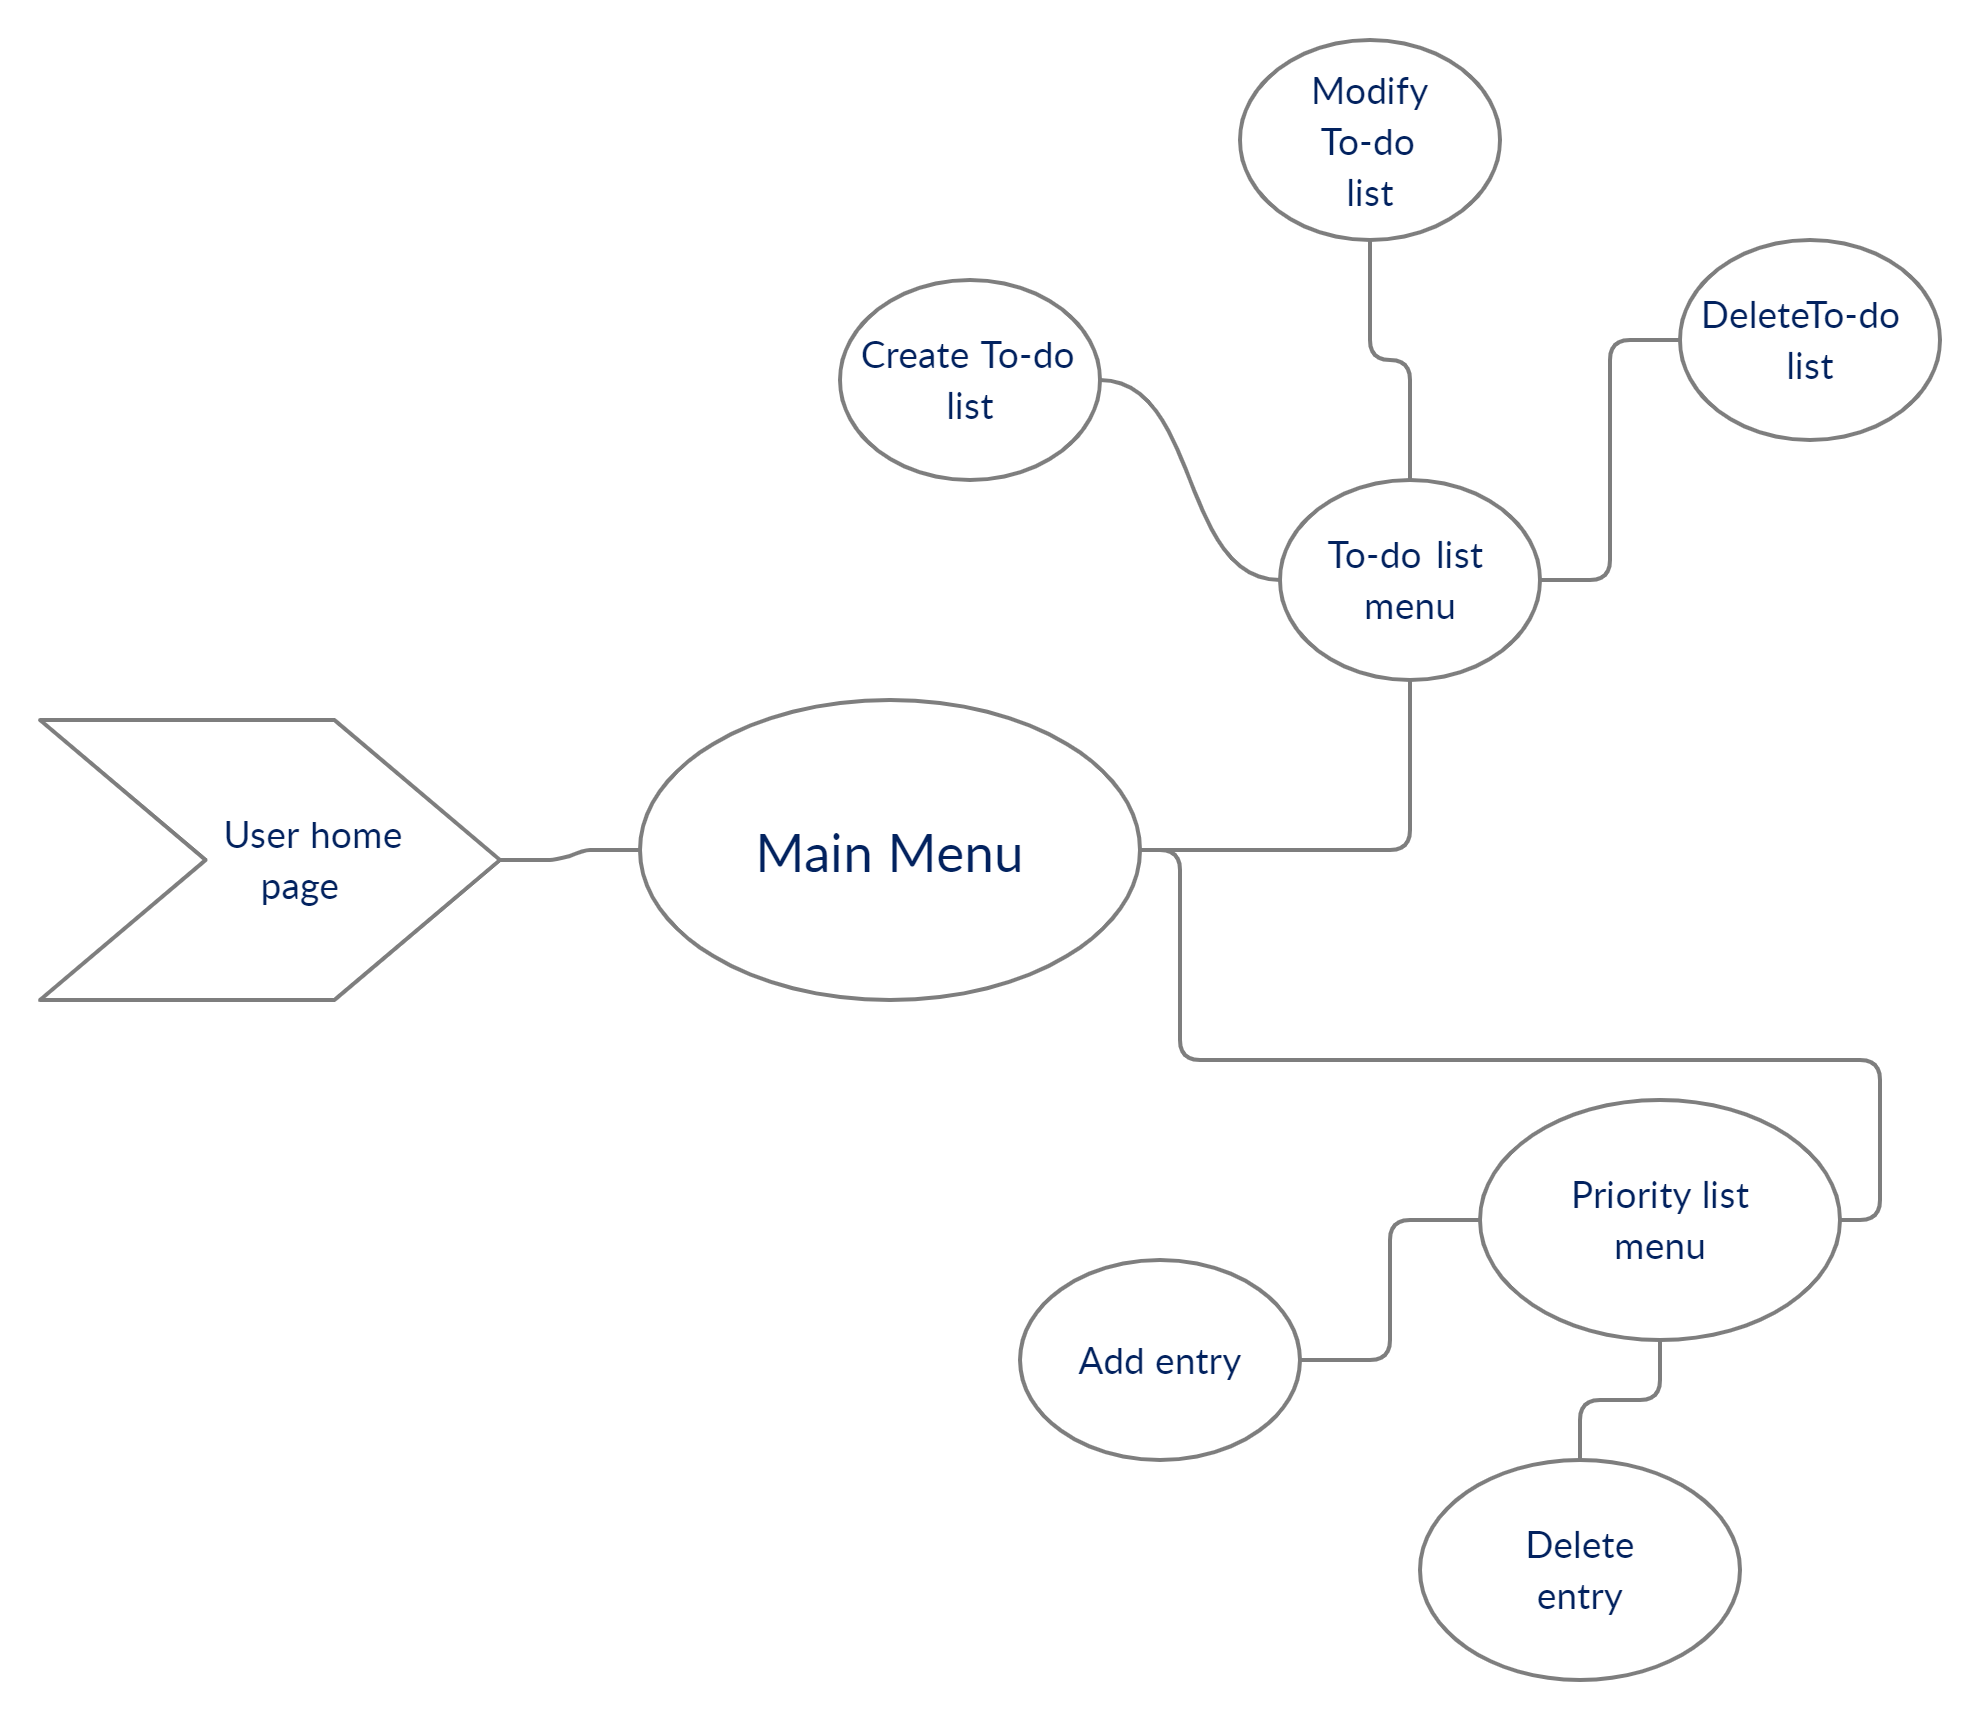
\includegraphics[width=\textwidth]{diagramusecase1}
	\caption{Use case diagram}
\end{figure}
\par In first Use case diagram we can see that a user can get multiple functionality of Main menu from home page, functionalities like to-do list and priority list with its functionalities.

\par
\begin{figure}[h]
	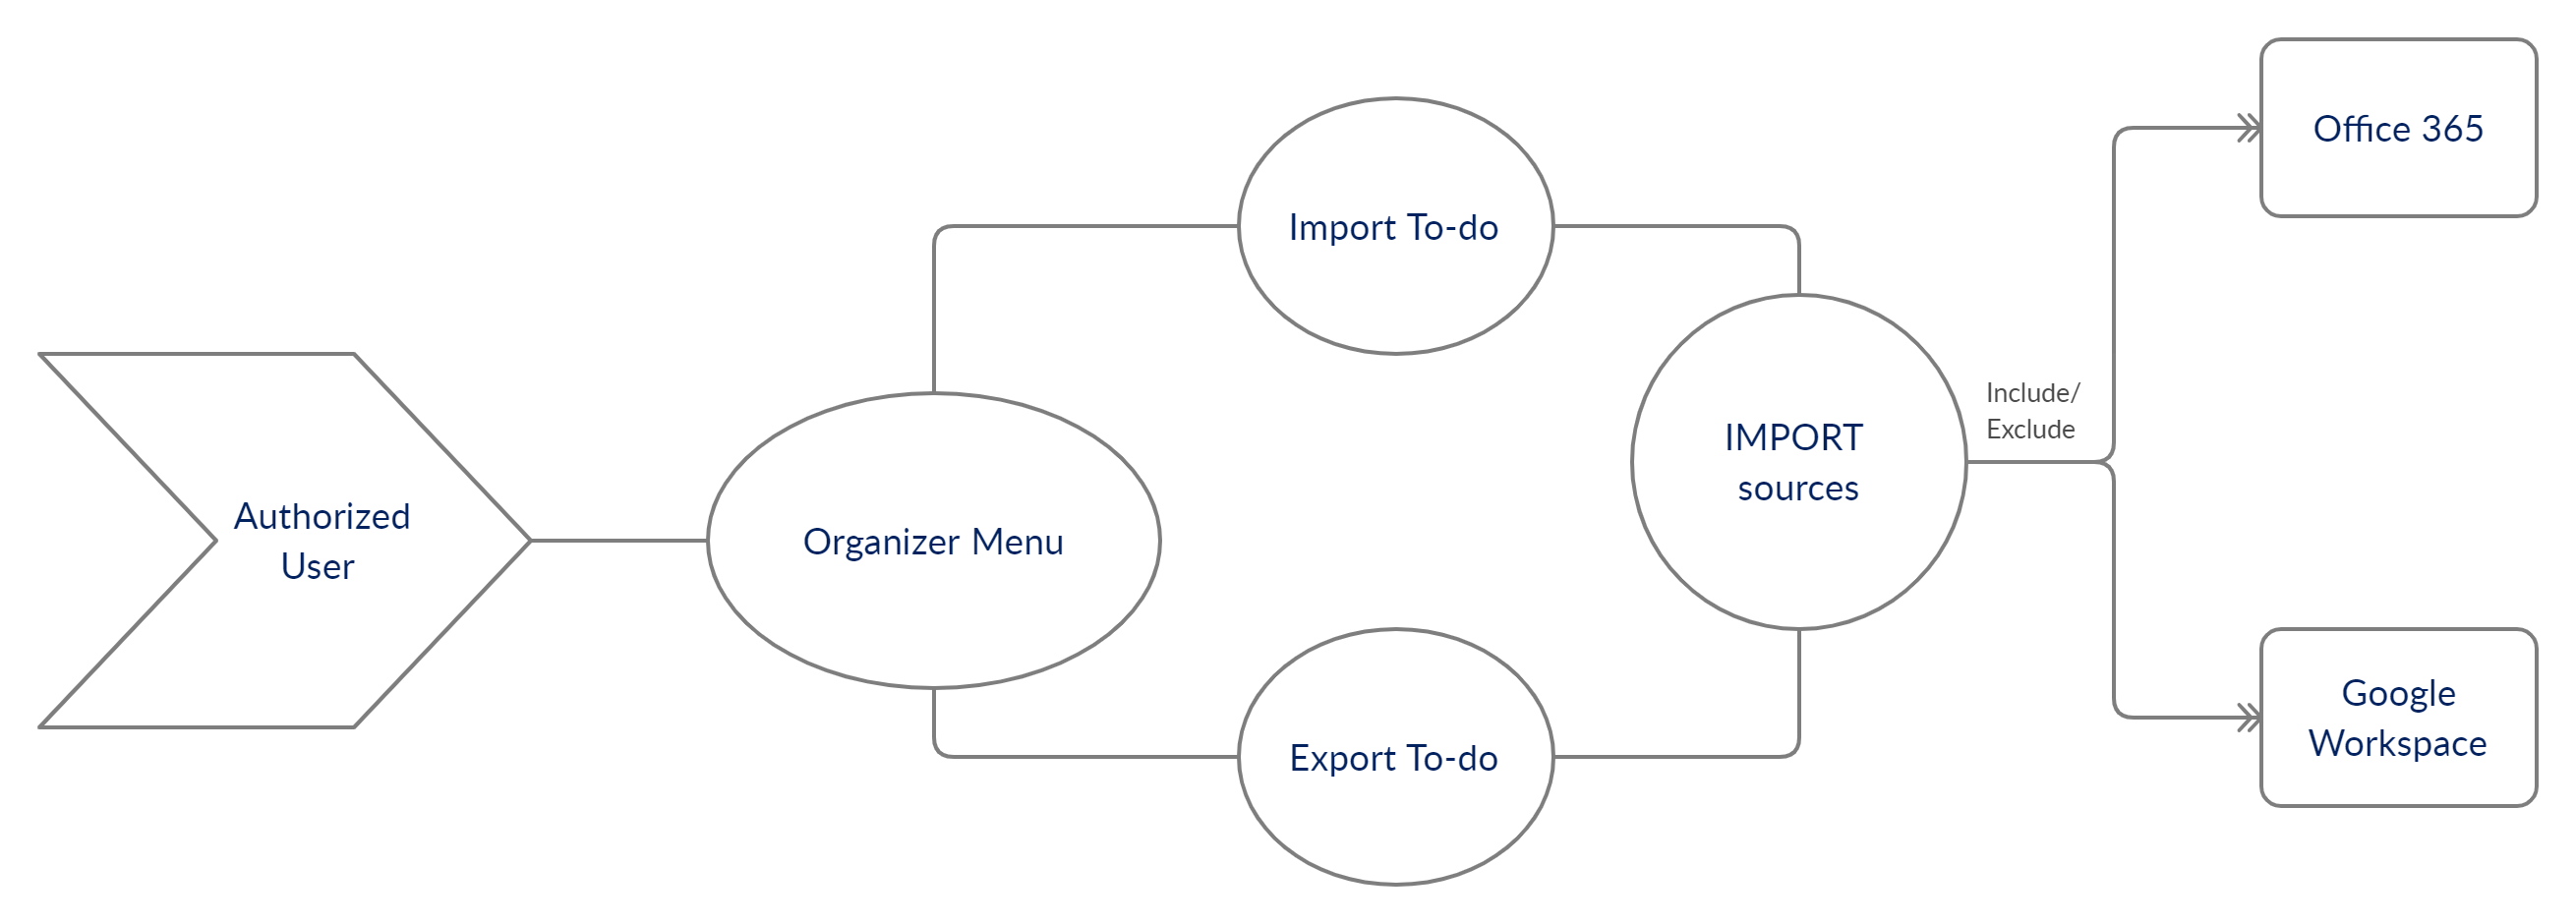
\includegraphics[width=\textwidth]{diagramusecase2}
	\caption{Use case diagram}
\end{figure}
\par In second Use case diagram user obtain the abilities to import or to export to-do list through organizer menu, user is capable of choosing the source of importing or exporting.
\subsubsection{Component}
\par
\begin{figure}[h]
	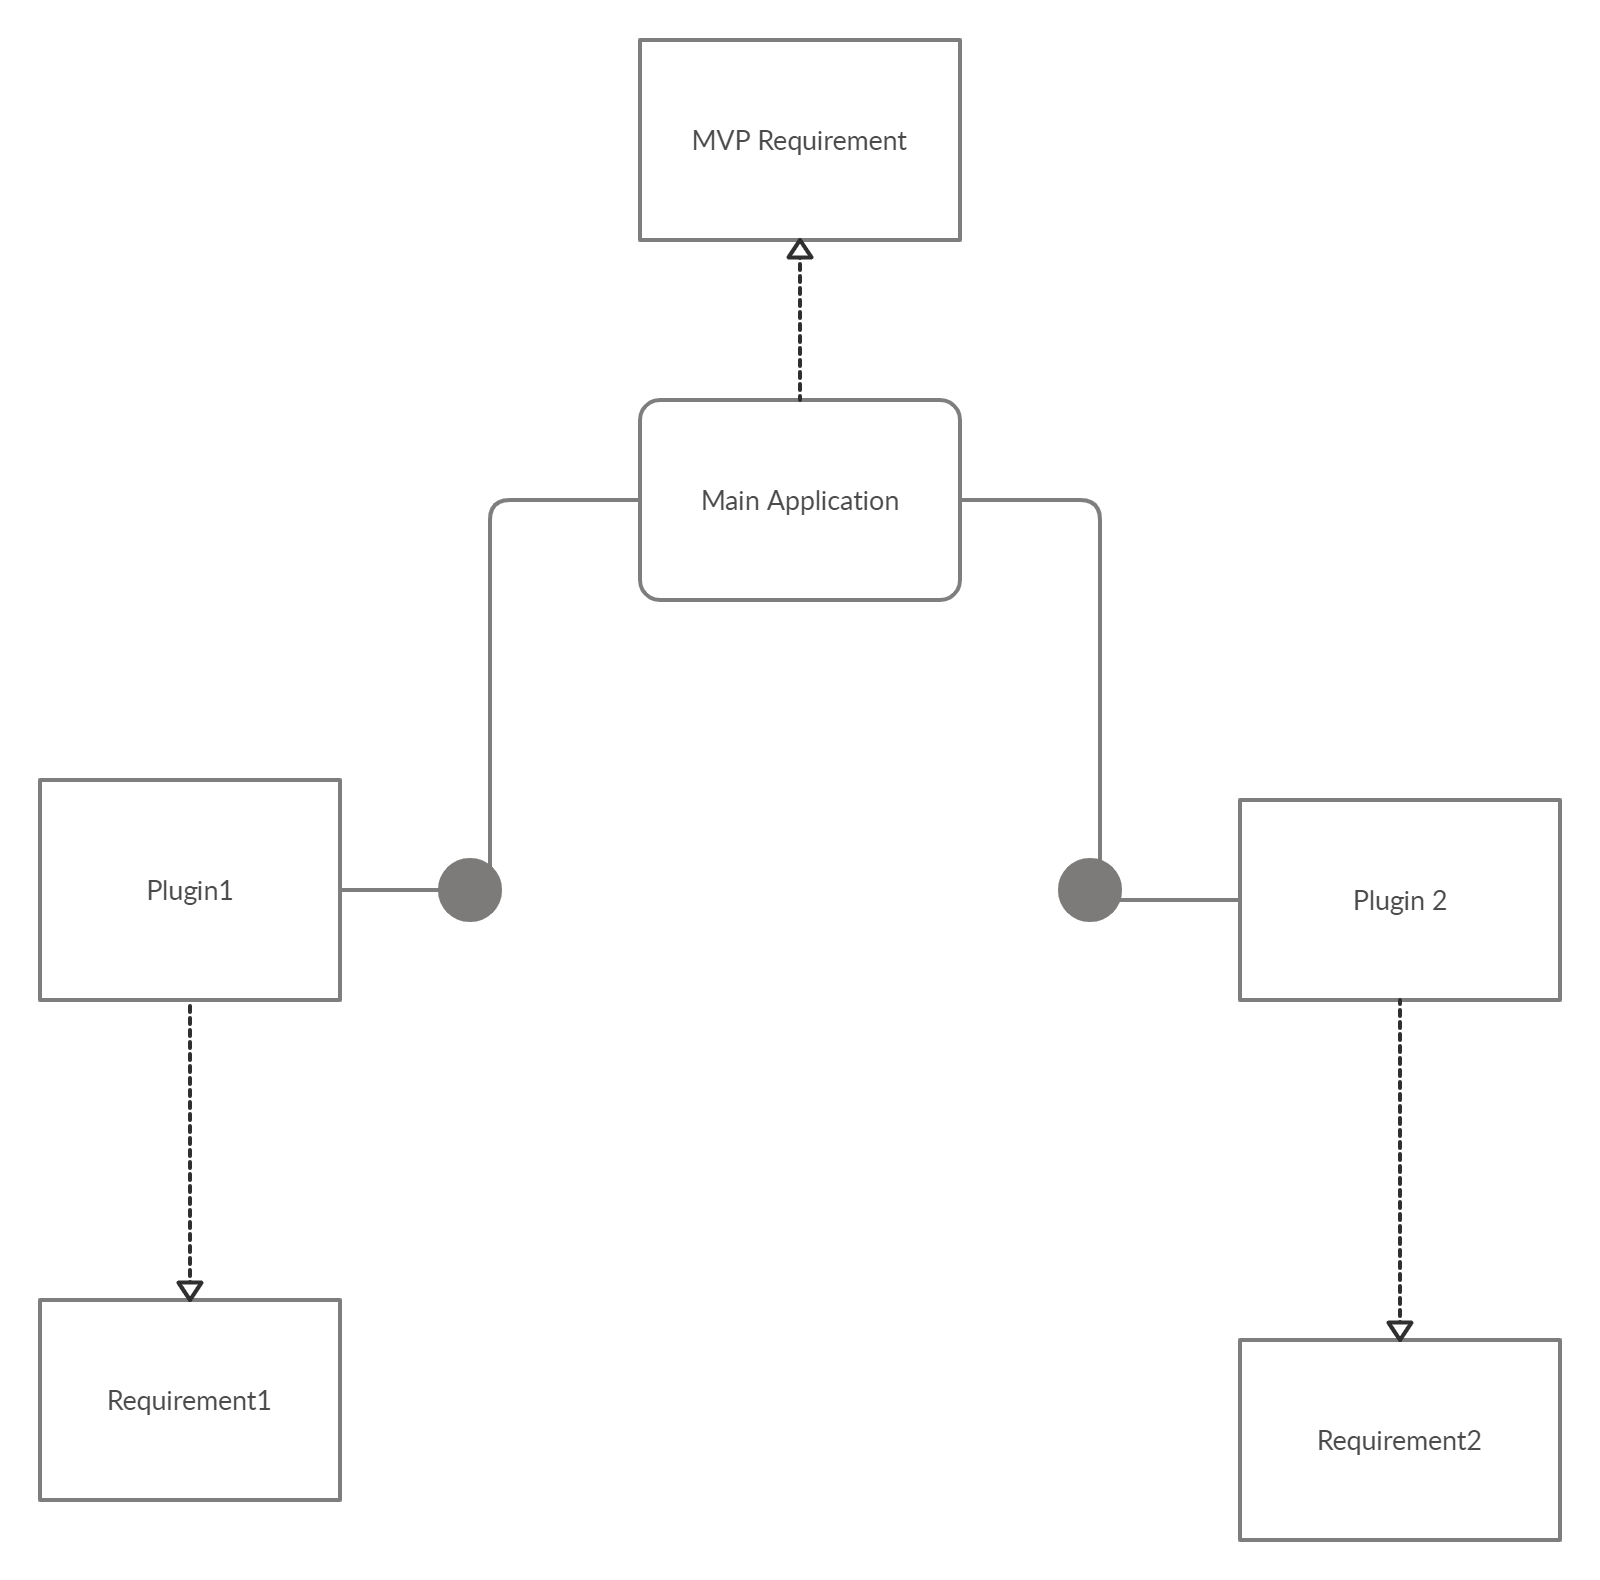
\includegraphics[width=\textwidth]{componentdigram1}	
	\caption{Component diagram}
\end{figure}
\par MVP Requirements are the Minimum Valuable Product Requirements that we established at the middle of semester: 
\begin{itemize}
	\item Custom plugins support like:weather, time, to-do list, map events
	\item Connection between frontend and backend
	\item User authentication and validation
	\item Agenda that contains all upcoming activities
	\item Dashboard that can be viewed in day, week, work week and month mode.
	
\end{itemize}

And according to this MVP we can have different modules of smaller parts of our application, based on plugins we want to implement and all requirements are linked to them as an example weather plugin which should be integrated with the help of an API.


\subsection{Sequence}
\par
\begin{figure}[h]
	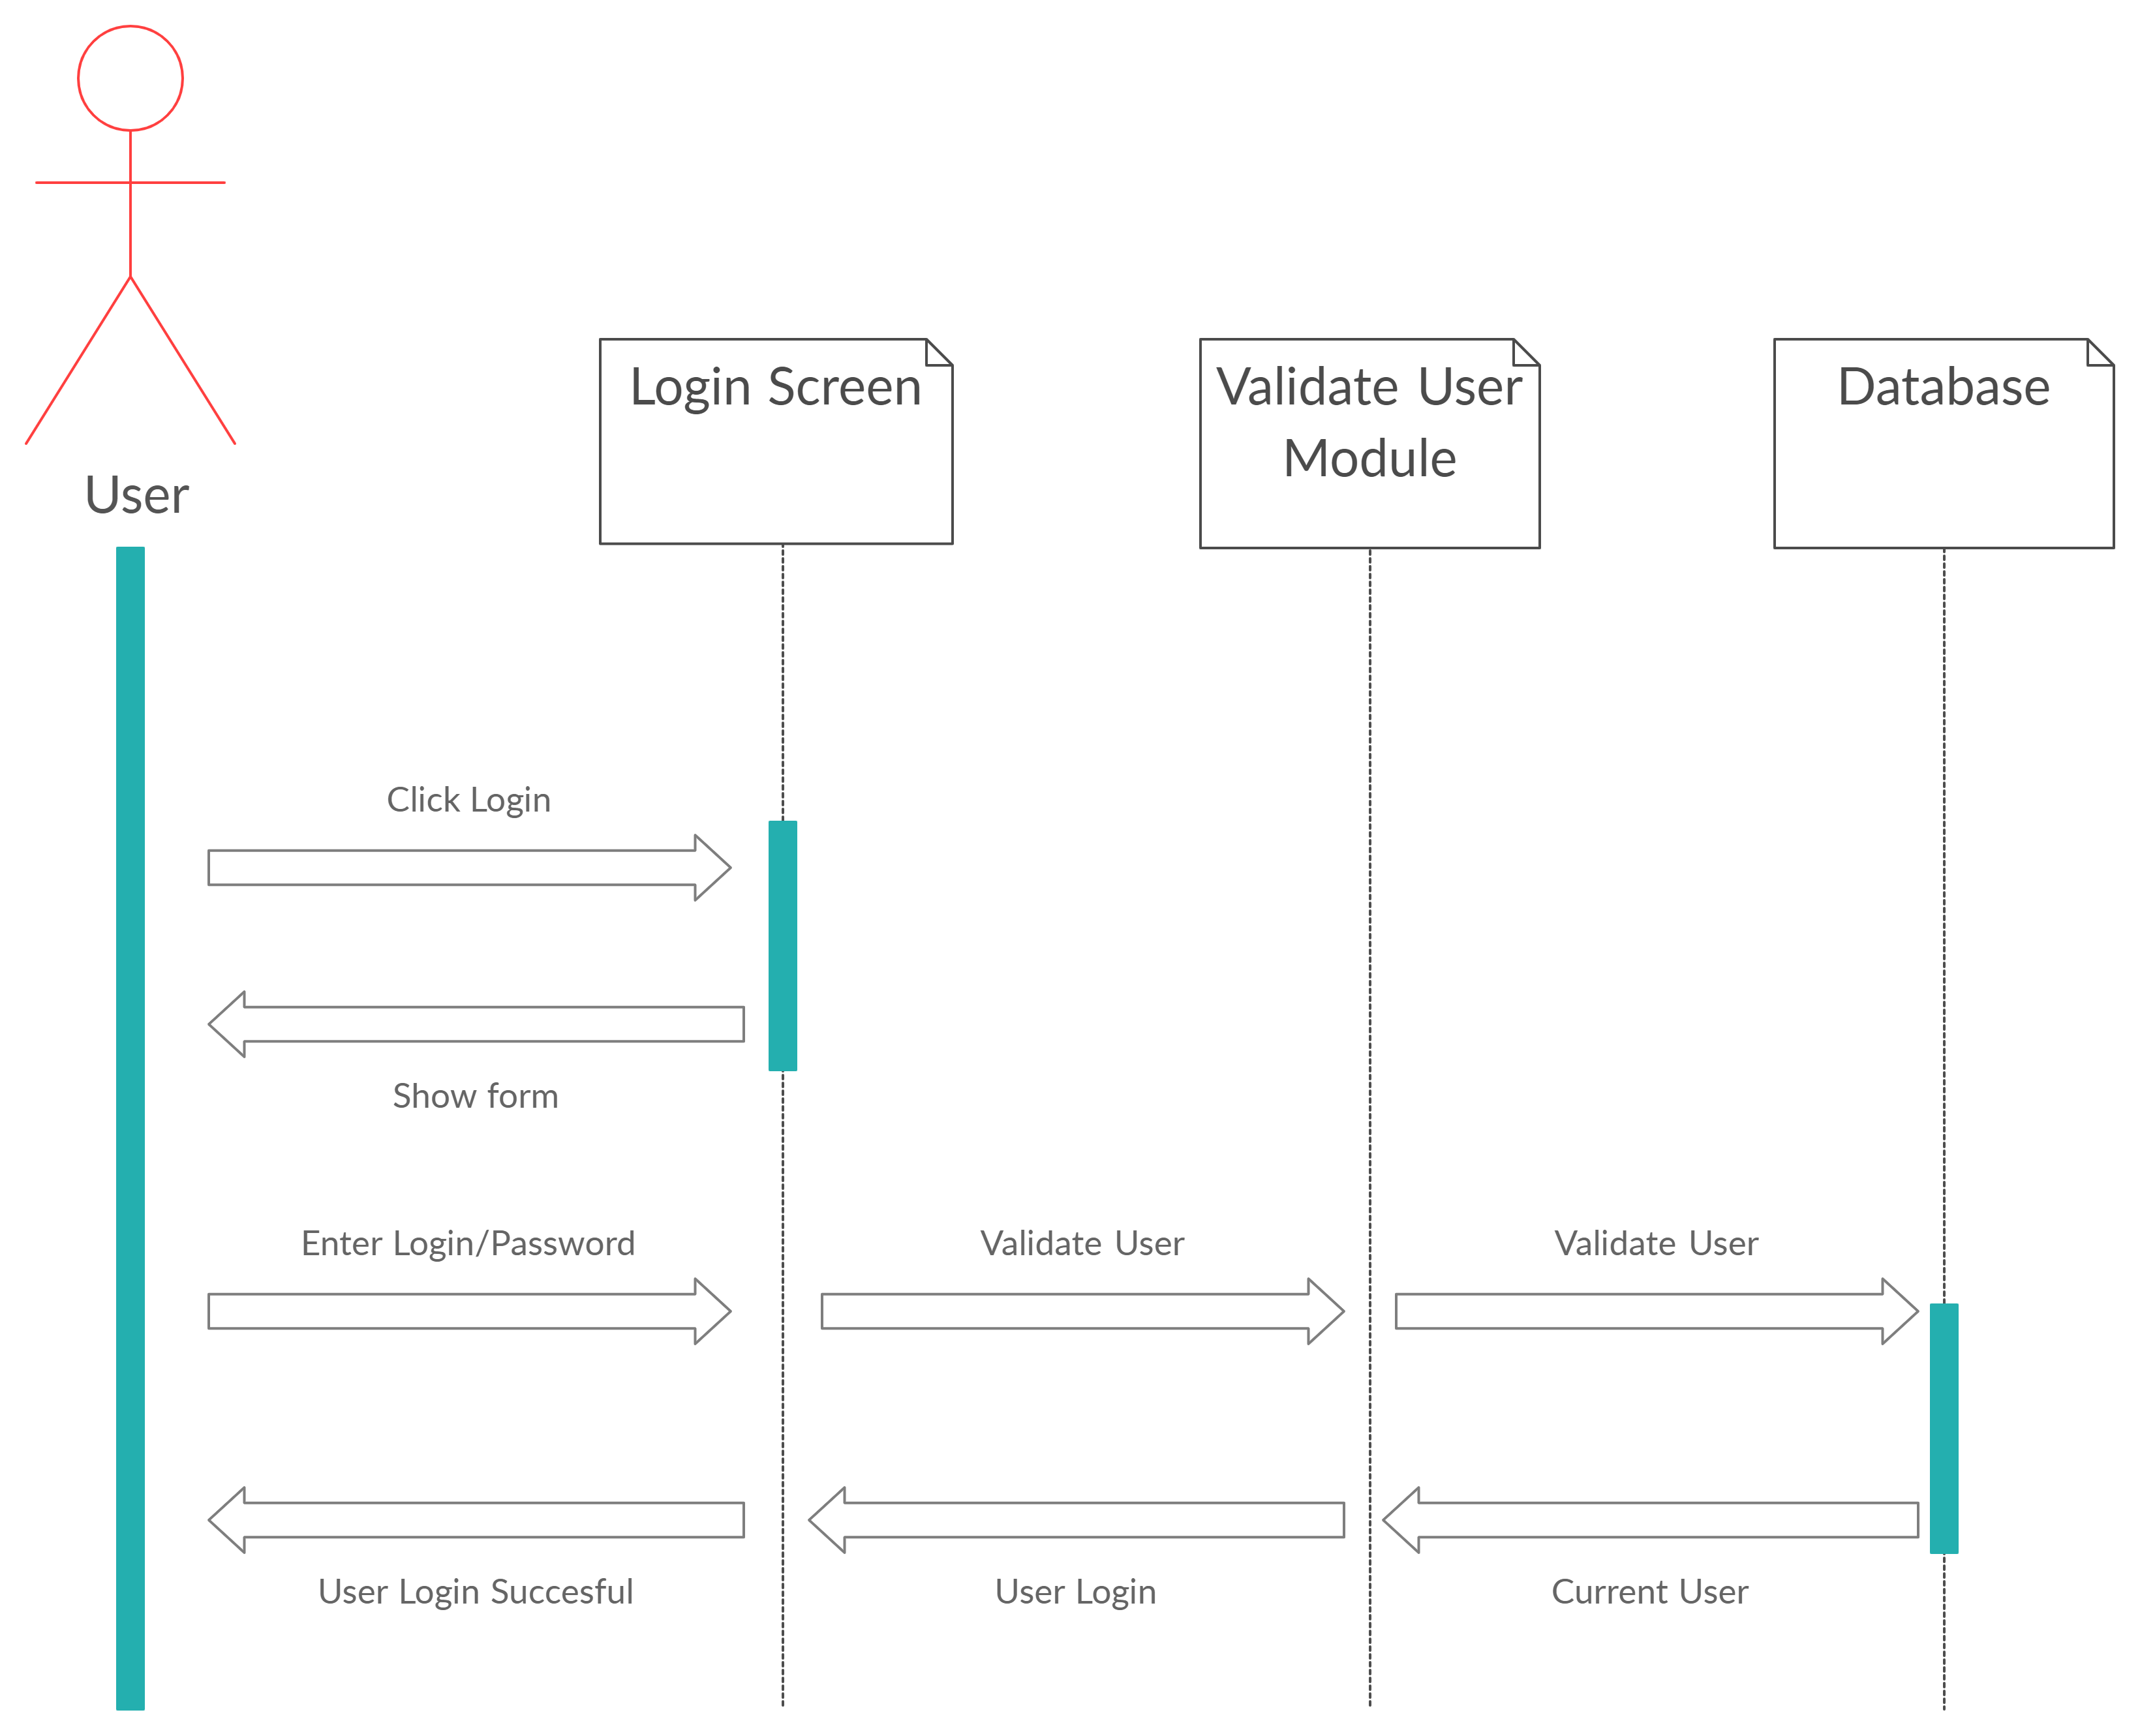
\includegraphics[width=\textwidth]{secuence digrram1}
	\caption{Sequence diagram}	
\end{figure}
\par In the following sequence diagram we are going to detail the interaction between components within login action. Suppose that it is a potential user that wants to login into our application. For the starting point he should access the signin form and complete it with credentials. These should be validated in the auth component by querying the database for that data. If data is validated the user is login successfully.
\par

\begin{figure}[h]
	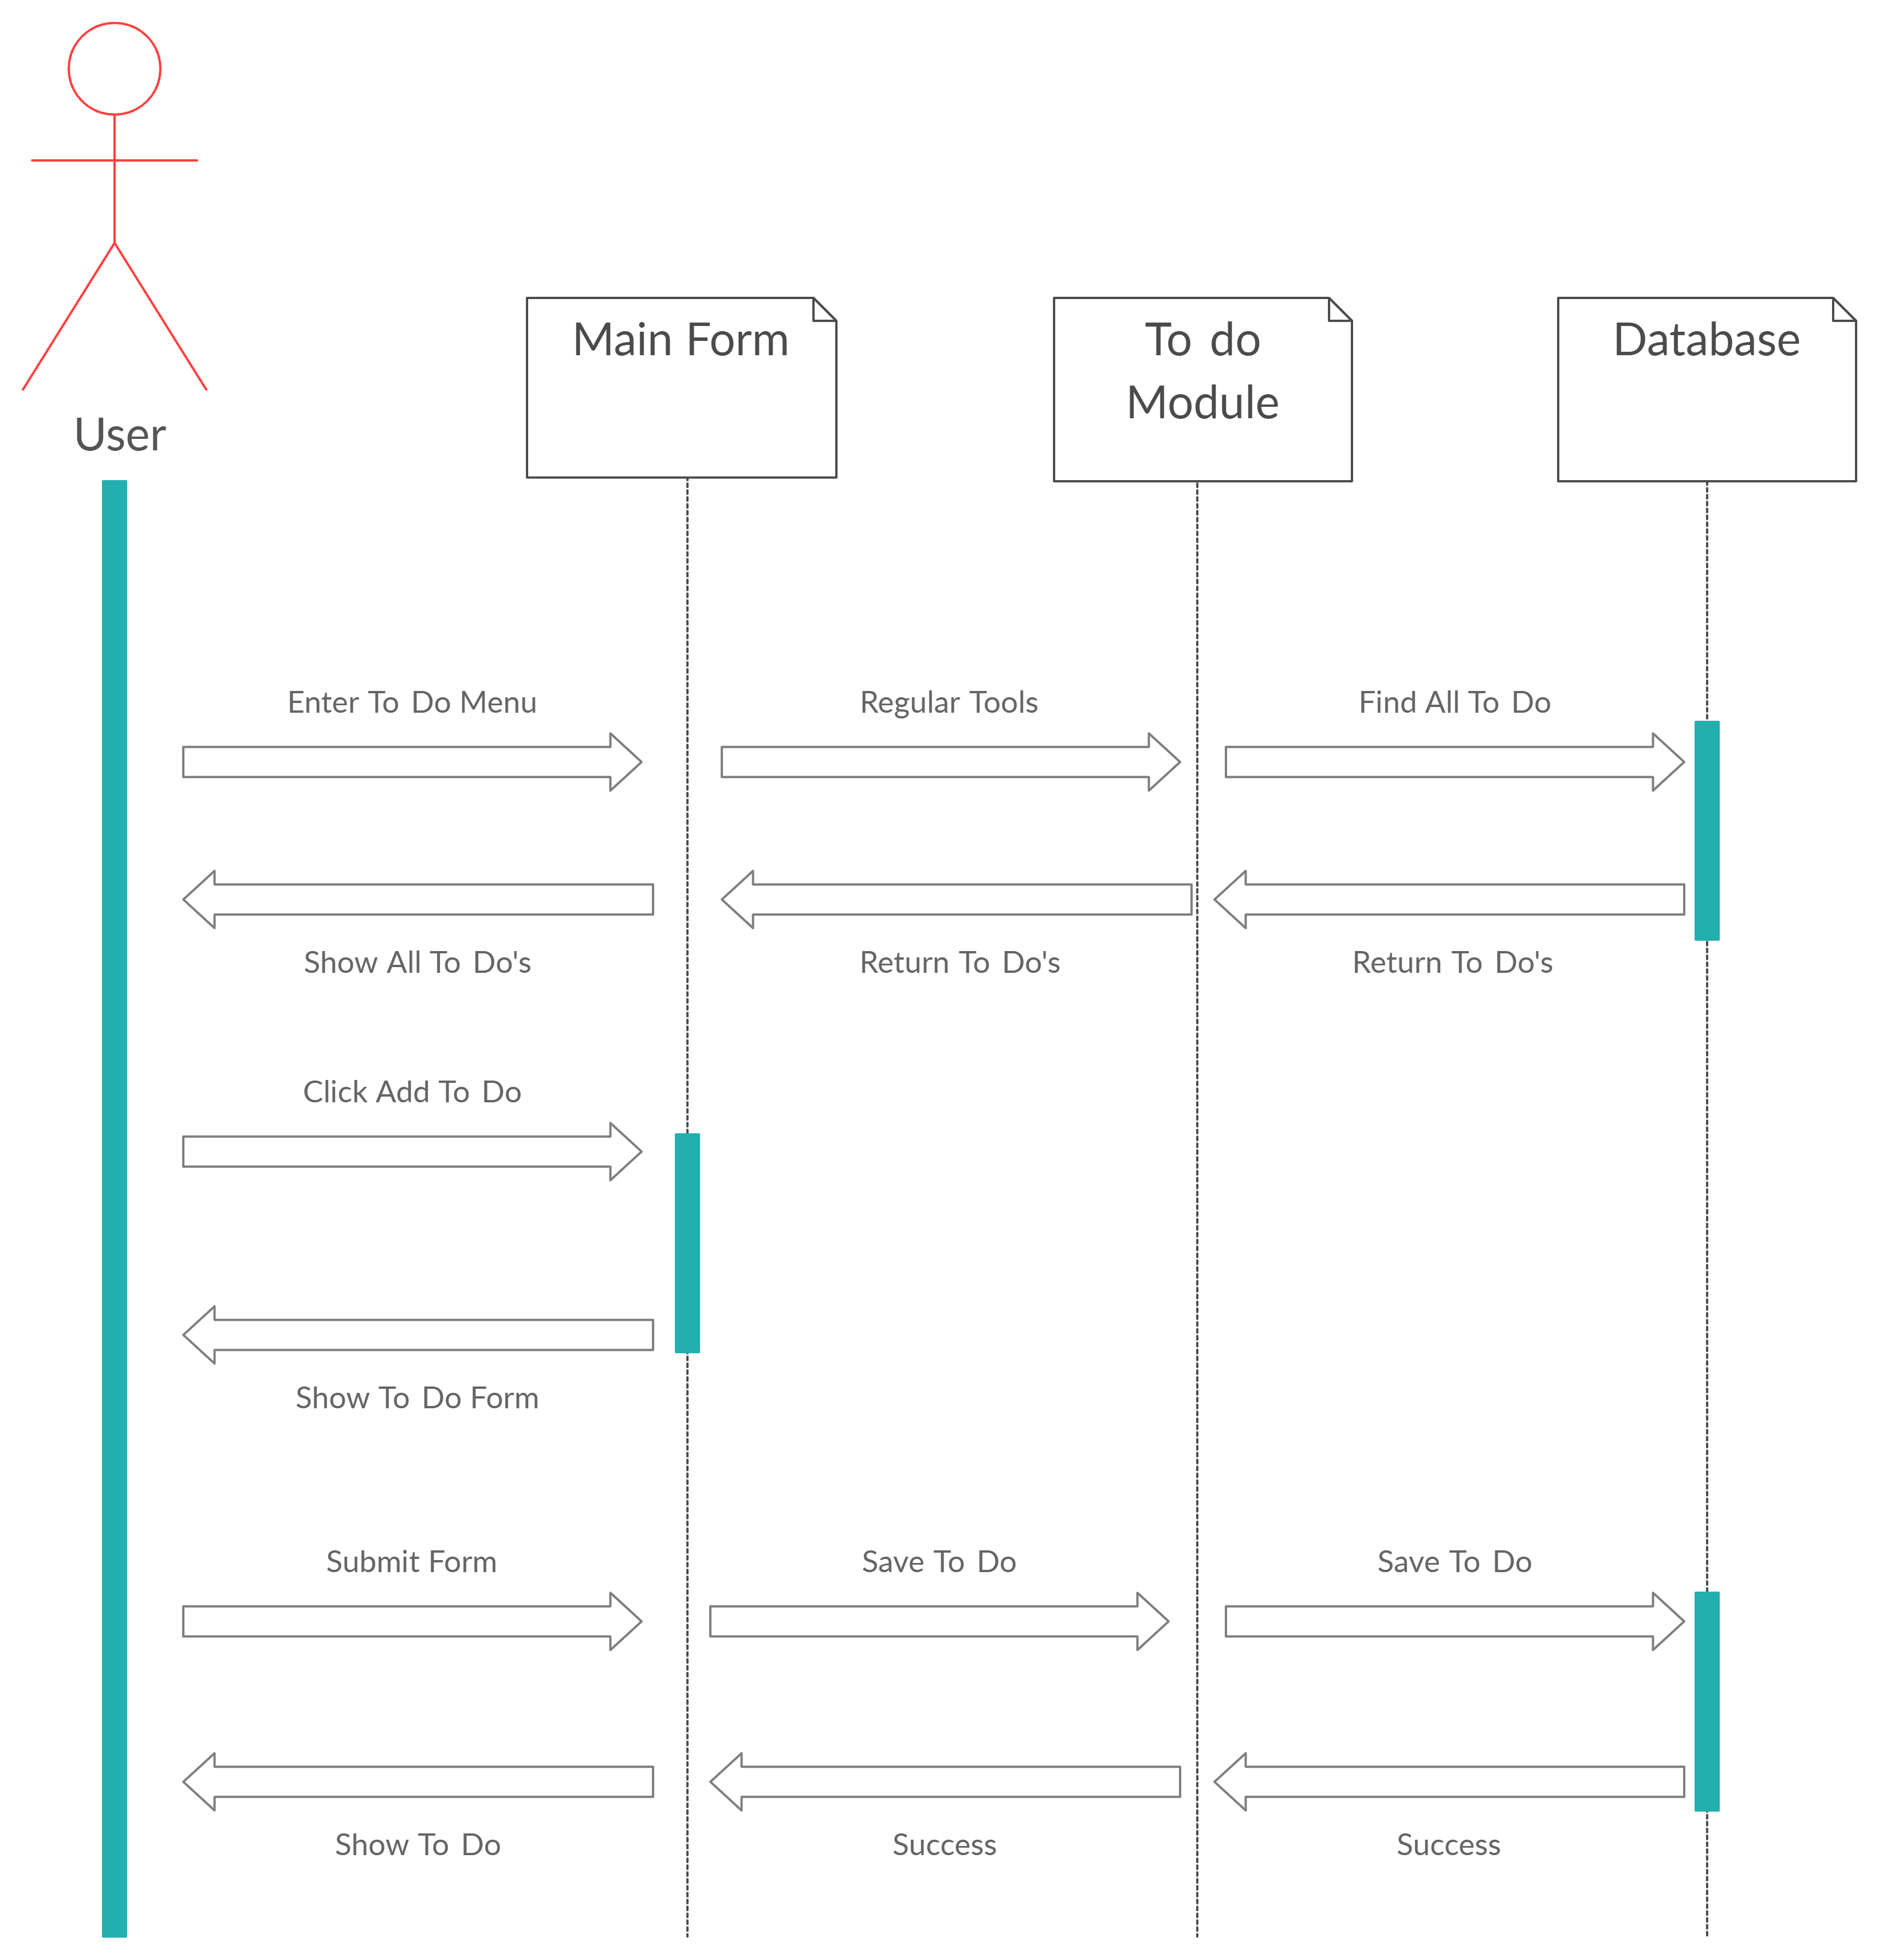
\includegraphics[width=\textwidth]{secuence digrram2}
	\caption{Sequence diagram}
\end{figure}
\par The second sequence diagram reflects the to-do plugin. The user should enter the to-do menu where he gets the list of all activities to complete from the database. He also can add and modify new events  from to-do form by adding them to the database and showing them afterwards.
\par 
\begin{figure}[h]
	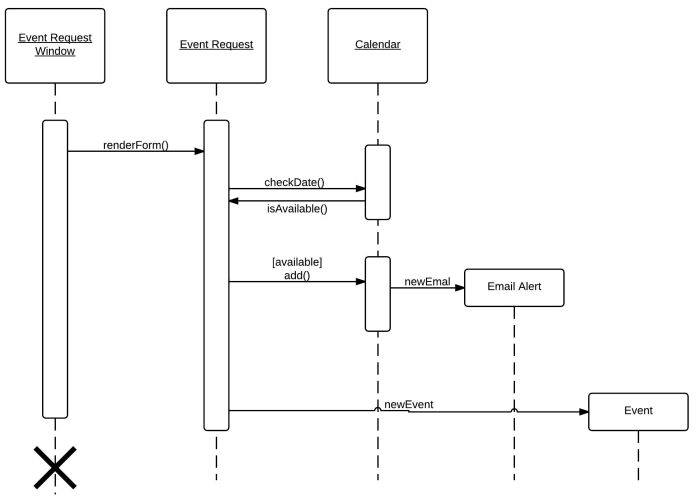
\includegraphics[width=\textwidth]{Sequence_Diagram3}
	\caption{Sequence diagram}	
\end{figure}
\par In the following sequence diagram we are going to detail the interaction between components within the Event requesting process. Every user then wants to create and introduce an event in the calendar has to open an event request window where he introduces information about time and description of this event, after request is checking the disponibility of this date, if an available event is introduced in the calendar. After the event is added an email alert is created which says details about the event. 

\par 
\begin{figure}[h]
	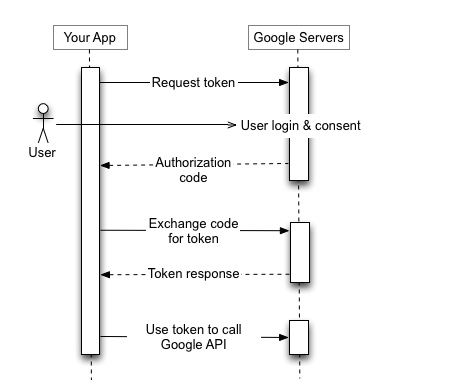
\includegraphics[width=\textwidth]{Sequence_Diagram4}
	\caption{Sequence diagram}	
\end{figure}


\par (2)The authorization sequence begins when  application redirects a browser to a Google URL; the URL includes query parameters that indicate the type of access being requested. Google handles the user authentication, session selection, and user consent. The result is an authorization code, which the application can exchange for an access token and a refresh token.

The application should store the refresh token for future use and use the access token to access a Google API. Once the access token expires, the application uses the refresh token to obtain a new one.

\subsection{Activity}
\par
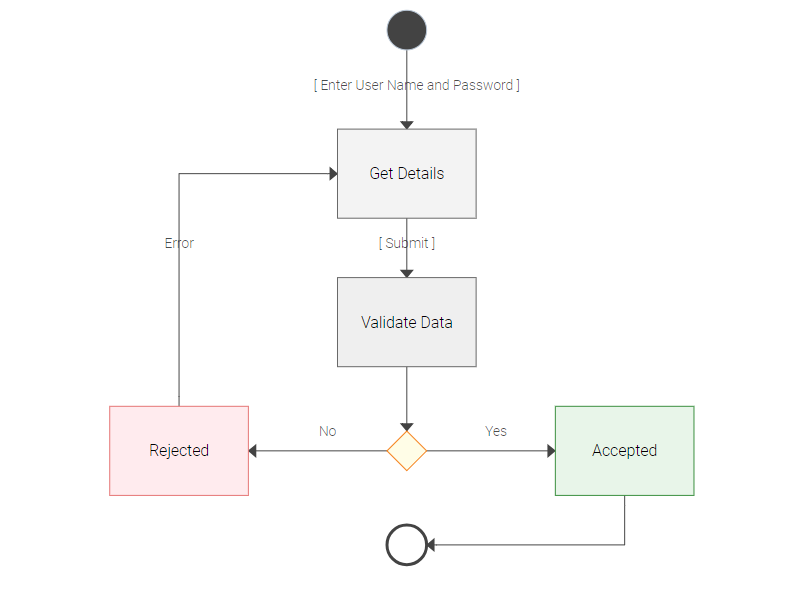
\includegraphics[width=\textwidth]{Activity_Diagram}
\subsection{Class}
\par
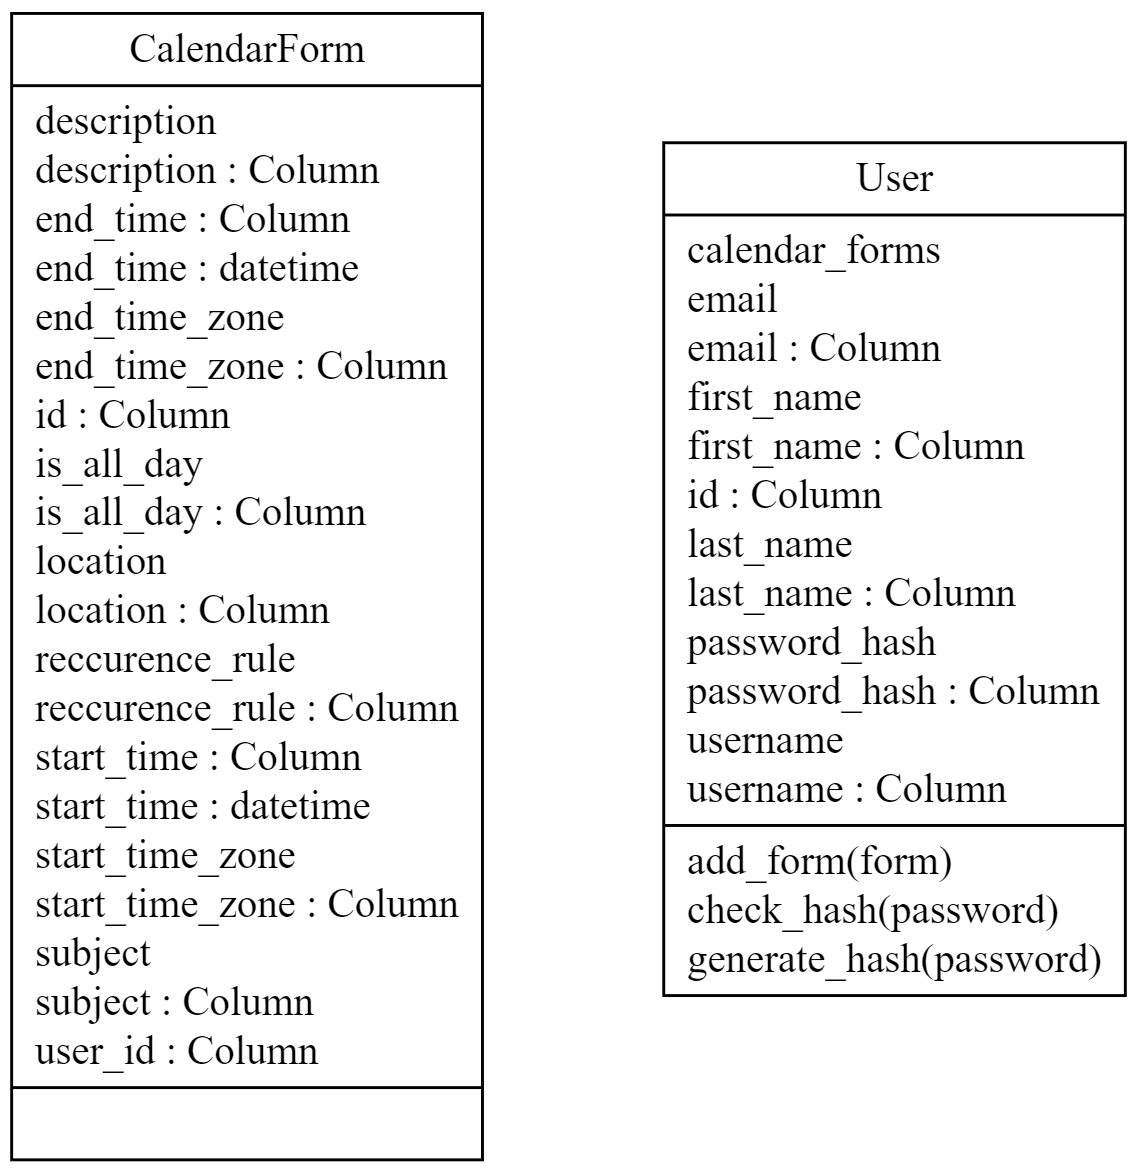
\includegraphics[width=\textwidth]{ClassDigram2}
\par 
\begin{figure}[htbp]
	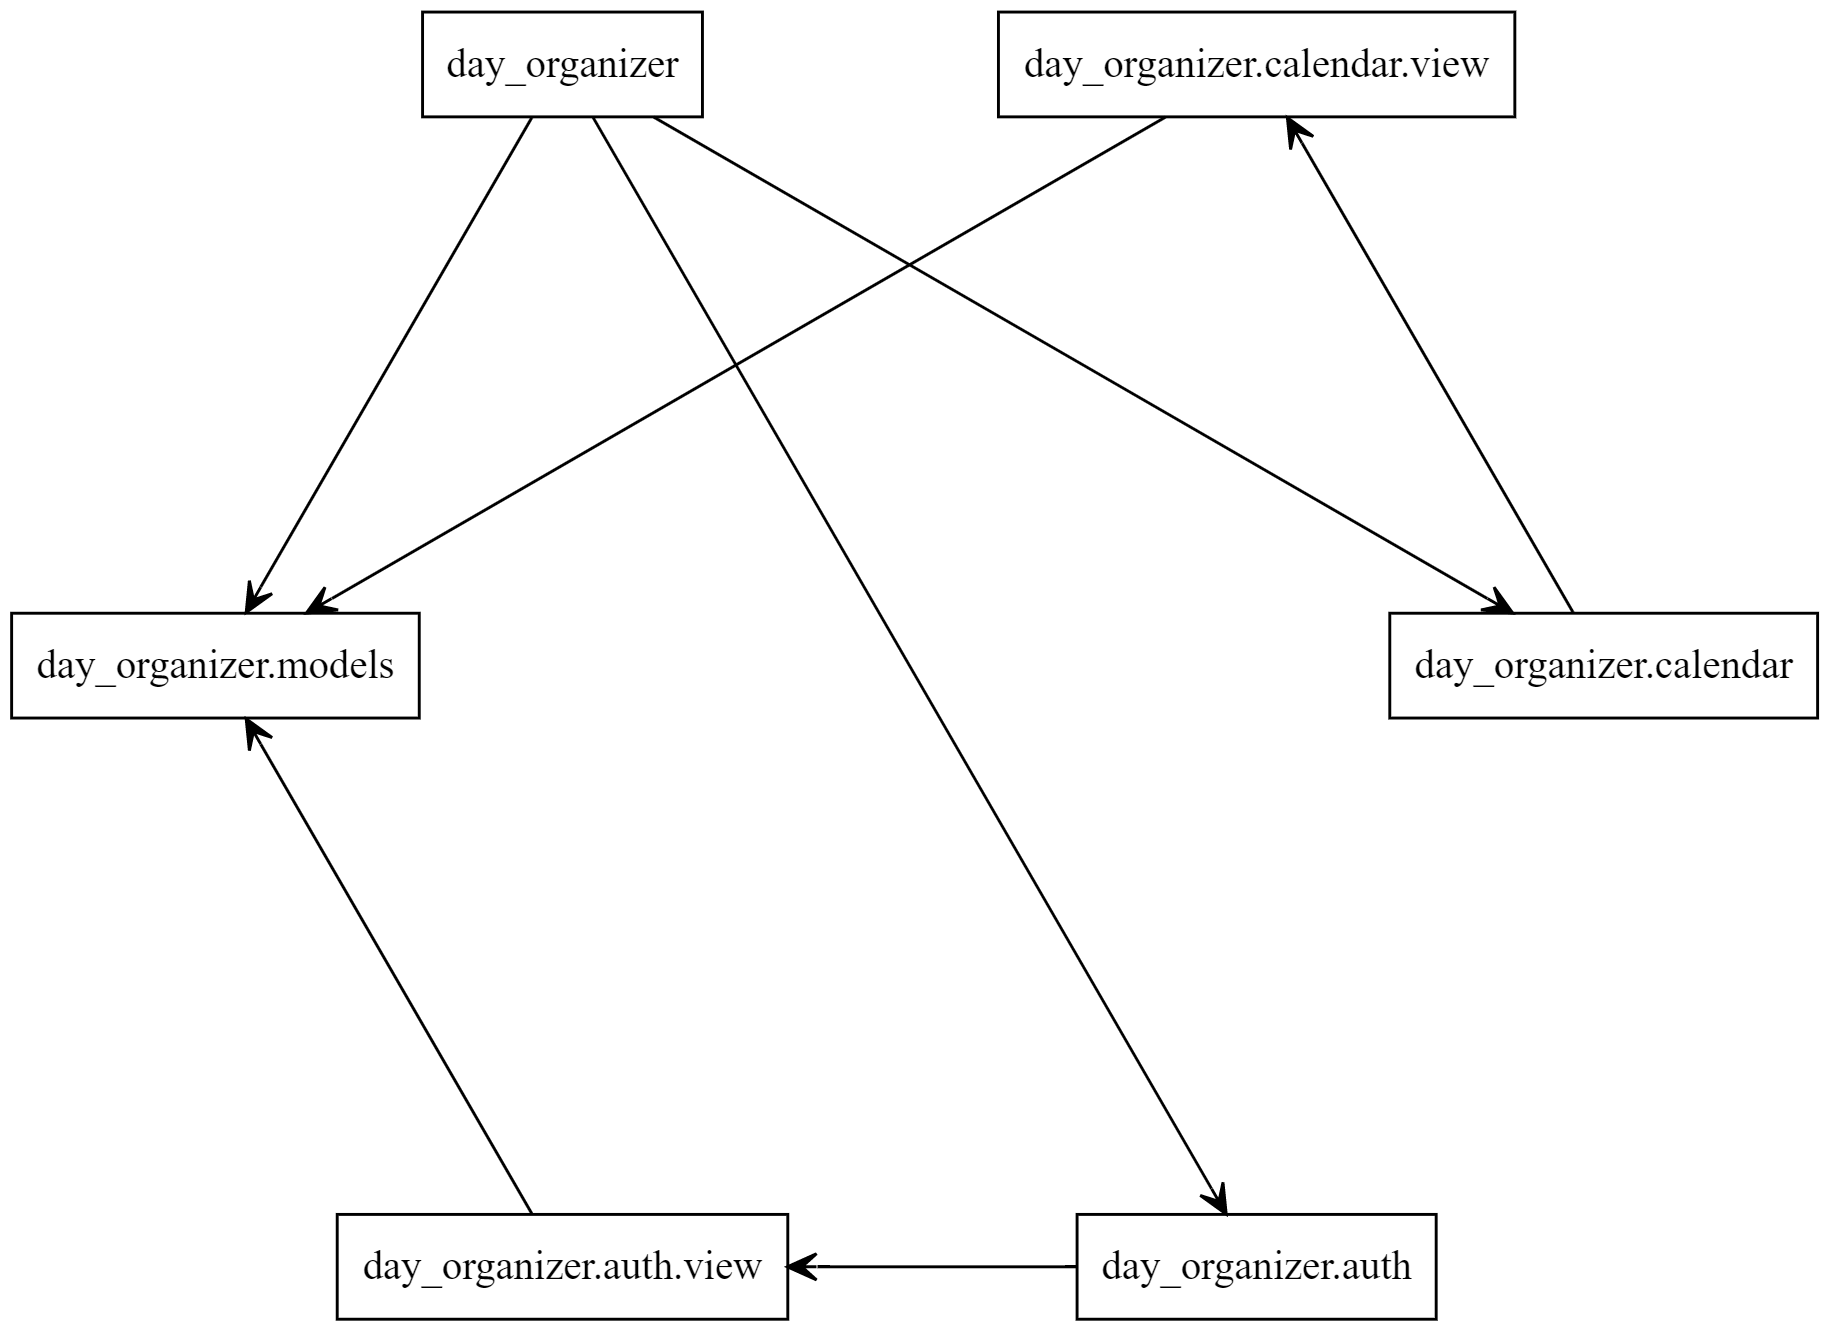
\includegraphics[width=\textwidth] {ClassDigram3}
	\caption{Class diagram}	
\end{figure}

\par The following class diagram reflects how the main components interact with each other. day\underline{ }organizer is the main namespace that contains day\underline{ }organizer.models, day\underline{ }organizer.auth, day\underline{ }organizer.calendar, day\underline{ }organizer.plugins, day\underline{ }organizer.plugins, day\underline{ }organizer.models.py.And all these components contains \underline{ }init\underline{ }.py and view.py files accordingly.


\clearpage